\documentclass[aspectratio=169]{beamer}
\usepackage{beamerthemesplit}
\usepackage{wrapfig}
\usetheme{SPbGU}
\usepackage{pdfpages}
\usepackage{amsmath}
\usepackage{cmap} 
\usepackage[T2A]{fontenc} 
\usepackage[utf8]{inputenc}
\usepackage[english,russian]{babel}
\usepackage{indentfirst}
\usepackage{amsmath}
\usepackage{tikz}
\usepackage{multirow}
\usepackage{subcaption}
\usepackage[noend]{algpseudocode}
\usepackage{algorithm}
\usepackage{algorithmicx}
\usetikzlibrary{shapes,arrows,fit,calc,automata,positioning}
\usepackage{fancyvrb}
\newtheorem{rutheorem}{Теорема}
\newtheorem{task}{}
\newtheorem{ruproof}{Доказательство}
\newtheorem{rudefinition}{Определение}
\newtheorem{rulemma}{Лемма}
\beamertemplatenavigationsymbolsempty

\title[]{Реализация и экспериментальное исследование GLL-парсера, основанного на рекурсивном автомате}
% То, что в квадратных скобках, отображается в левом нижнем углу. 
\institute[СПбГУ]{
Санкт-Петербургский государственный университет \\
Кафедра системного программирования }

% То, что в квадратных скобках, отображается в левом нижнем углу.
\author[Абзалов Вадим]{Абзалов Вадим Игоревич, 19.Б11-мм \\
  % У научного руководителя должна быть указана научная степень
  \and  
    {\bfseries Научный руководитель:} к.\,ф.-м.\,н., доцент кафедры информатики Григорьев С.\,В. \\ 
  % Для курсовой не обязателен. Должна быть указана должность или ученая степень
}
\date{19 мая 2023г.}

\definecolor{orange}{RGB}{179,36,31}

\begin{document}
{
% Лого университета или организации, отображается в шапке титульного листа
\begin{frame}
  \begin{center}
  {
\includegraphics[width=1.2cm]{pictures/SPbGU_Logo.png}}
  \end{center}
  \titlepage
\end{frame}
}

\begin{frame}[fragile]
  \transwipe[direction=90]
  \frametitle{Введение}
  \begin{itemize}
      \item Графовая модель представления данных
      \begin{itemize}
        \item Основные сущности --- вершины графа
        \item Взаимосвязи между сущностями хранятся в самой графовой модели
      \end{itemize}
\item Ограничения в виде формальных грамматик
\begin{itemize}
    \item Наибольшее применение находят регулярные и контекстно-свободные грамматики
    \item Имеют широкое применение в биоинформатике, анализе RDF-файлов
\end{itemize}
\item GLL алгоритм не позволяет напрямую работать с регулярными выражениями
\item Рекурсивные автоматы поддерживают как регулярные, так и контестно-свободные грамматики
\end{itemize}
\end{frame}

\begin{frame}[fragile]
  \transwipe[direction=90]
  \frametitle{Задача поиска путей с контекстно-свободными ограничениями}
   \begin{task}
  Дано:
     \begin{itemize}
    \item Контекстно-свободная грамматика $\mathbb{G}  = \langle N, \Sigma, P, S \rangle$
     \item Ориентированный граф $ \mathbb{D} = \langle V, E, T \rangle$
     \item Множество стартовых вершин $V_S \subseteq V$  и финальных вершин \mbox{$V_F \subseteq V$}
\end{itemize} 
\textbf{Задача поиска путей}:
\begin{itemize}
    \item Найти все такие пути $\pi = (e_0, e_1, \cdots, e_{n - 1}, e_n), ~ e_k = (v_{k - 1}, t_k, v_k)$ в графе $ \mathbb{D}$, что $l(\pi) = t_1t_2 \cdots t_n \in L(\mathbb{G})$ и $v_0 \in V_S, ~v_n \in V_F$
\end{itemize}
\textbf{Задача поиска достижимостей}:
\begin{itemize}
    \item Найти множество пар $\{(v_i, v_j ) ~|~ \exists ~\pi : ~l(\pi) \in L(\mathbb{G})$ и $v_0 \in V_S, ~v_n \in V_F\}$
\end{itemize}
 \end{task}
\end{frame}

\begin{frame}
  \transwipe[direction=90]
  \frametitle{Цели и задачи}
  \textbf{Целью} данной работы является реализация и экспериментальное исследование производительности GLL алгоритма, основанного на рекурсивном автомате
  
  \textbf{Задачи}:
  \begin{itemize}
    \item Реализация классического GLL алгоритма
    \item Модификация алгоритма GLL для поддержки представления грамматики в виде рекурсивного автомата
    \item Расширение модифицированного алгоритма GLL на входные данные в виде графа
    \item Проведение экспериментального исследования и сравнение с существующими решениями
\end{itemize}
\end{frame}

\begin{frame}
  \transwipe[direction=90]
  \frametitle{Обзор GLL алгоритма}
  \textbf{Обобщенный LL-алгоритм (GLL)}
\begin{itemize}
    \item Поддерживает весь класс контекстно-свободных языков
    \item Для восстановления путей поддерживается сжатое представление леса разбора (SPPF)
    \item Обобщается на входные данные в виде графов
\end{itemize}
  \end{frame}

% \begin{frame}
% \transwipe[direction=90]
%  \frametitle{Реализация}
% \begin{itemize}
%     \item 
% \end{itemize}
% \end{frame}


\begin{frame}
\transwipe[direction=90]
 \frametitle{Архитектура}
 \begin{figure}[H]
\centering
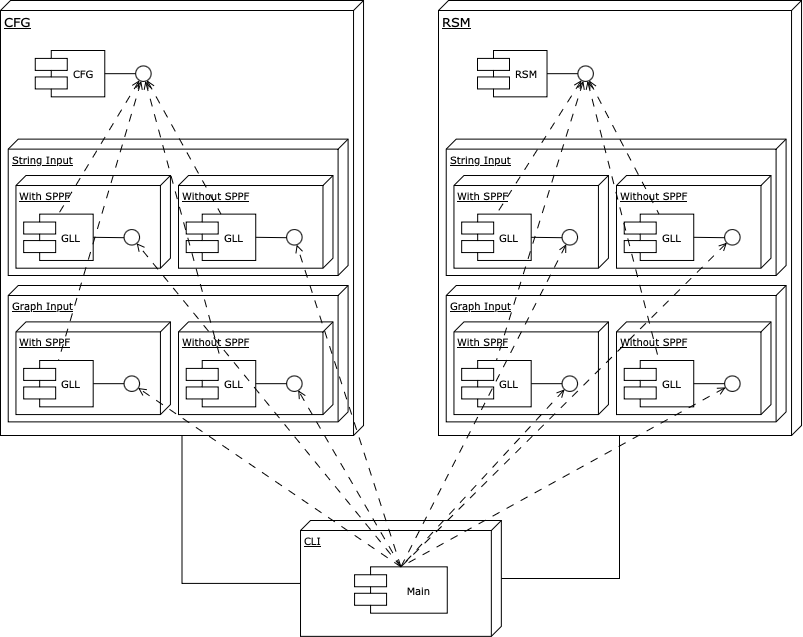
\includegraphics[width=0.55\textwidth]{SlidesTemplate/pictures/architecture.png}
\caption{Архитектура проекта}
% \includegraphics[width=0.9\textwidth]{SlidesTemplate/pictures/...pdf}
% \caption{}
% \label{fig:...}
\end{figure}
\end{frame}

\begin{frame}
  \transwipe[direction=90]
  \frametitle{Экспериментальное исследование полученного решения}

  \begin{figure}[H]
  \centering
  \begin{table*}
    \resizebox{\columnwidth}{!}{%
    \begin{tabular}{| l | r | r | r | r | r | r |}
         \hline
         Название графа & $|V|$ & $|E|$ & \#subClassOf & \#type & \#broaderTransitive\\
         \hline
         \hline
            % skos & 144 & 252 & 1 & 70 & 0 \\
            % generations & 129 & 273 & 0 & 78 & 0 \\
            % travel & 131 & 277 & 30 & 90 & 0 \\
            % univ & 179 & 293 & 36 & 84 & 0 \\
            % atom & 291 & 425 & 122 & 138 & 0 \\
            % biomedical & 341 & 459 & 122 & 130 & 0 \\
            % foaf & 256 & 631 & 10 & 174 & 0 \\
            % people & 337 & 640 & 33 & 161 & 0 \\
            % funding & 778 & 1086 & 90 & 304 & 0 \\
            % wine & 733 & 1839 & 126 & 485 & 0 \\
            % pizza & 671 & 1980 & 259 & 365 & 0 \\
            % core & 1323 & 2752 & 178 & 706 & 0 \\
            % pathways & 6238 & 12363 & 3117 & 3118 & 0 \\
            enzyme & 48815 & 86543 & 8163 & 14989 & 8156 \\
            eclass & 239111 & 360248 & 90962 & 72517 & 0 \\
            go\_hierarchy & 45007 & 490109 & 490109 & 0 & 0 \\
            go & 582929 & 1437437 & 94514 & 226481 & 0 \\
            geospecies & 450609 & 2201532 & 0 & 89062 & 20867 \\
            taxonomy & 5728398 & 14922125 & 2112637 & 2508635 & 0 \\
         \hline
    \end{tabular}%
    }
\end{table*}
\caption{Графы класса RDF: количество вершин, ребер и ребер с определенными метками}
\end{figure}
\end{frame}

\begin{frame}
  \transwipe[direction=90]
  \frametitle{Экспериментальное исследование полученного решения}
  \begin{figure}[H]
        \begin{align}
        \begin{split}
        \label{eqn:g_1}
        S \to & \overline{\textit{subClassOf}} \ \ S \ \textit{subClassOf} \mid \overline{\textit{type}} \ \ S \ \textit{type}\\   & \mid \overline{\textit{subClassOf}} \ \ \textit{subClassOf} \mid \overline{\textit{type}} \ \textit{type}
        \end{split}
        \tag{$G_1$}
        \end{align}
        \begin{align}
        \begin{tikzpicture}[node distance=2cm,shorten >=1pt,on grid,auto]
           \node[state, initial] (q_0)   {$0 \{S\}$};
           \node[state] (q_1) [above right=of q_0] {$1 \{S\}$};
           \node[state] (q_2) [right=of q_1] {$2 \{S\}$};
           \node[state, accepting] (q_3) [below right=of q_2] {$3 \{S\}$};
           \node[state] (q_4) [below right=of q_0] {$4 \{S\}$};
           \node[state] (q_5) [right=of q_4] {$5 \{S\}$};
           \path[->]
            (q_0) edge[bend left, left]  node {$\overline{subClassOf}$} (q_1)
            (q_1) edge  node {$S$} (q_2)
            (q_2) edge[bend left, right]  node {$subClassOf$} (q_3)
            (q_1) edge[left]  node {$subClassOf$} (q_3)
            (q_0) edge[bend right, left] node {$\overline{type}$} (q_4)
            (q_4) edge[below]  node {$S$} (q_5)
            (q_5) edge[bend right, right]  node {$type$} (q_3)
            (q_4) edge[left]  node {$type$} (q_3);
        \end{tikzpicture}
        \tag{$A_1$}
        \end{align}
    \caption{Контекстно-свободная грамматика $G_1$ и соответствующий ей рекурсивный автомат $A_1$}
   \end{figure}
\end{frame}

\begin{frame}
  \transwipe[direction=90]
  \frametitle{Экспериментальное исследование полученного решения}
  \begin{figure}[H]
        \begin{align}
        \begin{split}
        \label{reg:rdf_reg_4}
        type^* \ subClassOf^*
        \end{split}
        \tag{$R_4$}
        \end{align}
        \begin{align}
        \begin{split}
        \label{cfg:rdf_reg_4}
        S & \to A \ B \\
        A & \to type \ A ~|~ \varepsilon \\
        B & \to subClassOf \ B ~|~ \varepsilon \\
        \end{split}
        \tag{$G_{R_4}$}
        \end{align}
        \begin{align}
    \label{rsm:rdf_reg_4}
        \begin{tikzpicture}[node distance=4cm,shorten >=1pt,on grid,auto, x=20mm, y=20mm]
           \node[state, initial, accepting] (q_0)   {$0 \{S\}$};
           \node[state, accepting] (q_1) [right=of q_0]   {$1 \{S\}$};
           \path[->]
            (q_0) edge[out=30, in=150, looseness=4, above] node {$type$} (q_0)
            (q_0) edge node {$subClassOf$} (q_1)
            (q_1) edge[out=30, in=150, looseness=4, above] node {$subClassOf$} (q_1)
            ;
        \end{tikzpicture}
        \tag{$A_{R_4}$}
    \end{align}
    \caption{Регулярное выражение $R_4$, соответствующие ему контекстно-свободная грамматика $G_{R_4}$ и рекурсивный автомат $A_{R_4}$}
   \end{figure}
\end{frame}

\begin{frame}
\transwipe[direction=90]
\frametitle{Результаты}
\begin{figure}
    \centering
    % Please add the following required packages to your document preamble:
% \usepackage{multirow}
\begin{table}[]
\resizebox{\columnwidth}{!}{%
\begin{tabular}{|l|rrrrr|}
\hline
\multicolumn{1}{|c|}{\multirow{3}{*}{\begin{tabular}[c]{@{}c@{}}Название\\ графа\end{tabular}}} &
  \multicolumn{5}{c|}{Время в секундах} \\ \cline{2-6} 
\multicolumn{1}{|c|}{} &
  \multicolumn{3}{c|}{G1} &
  \multicolumn{2}{c|}{R4} \\ \cline{2-6} 
\multicolumn{1}{|c|}{} &
  \multicolumn{1}{c|}{CFG} &
  \multicolumn{1}{c|}{RSM} &
  \multicolumn{1}{c|}{GLL4Graph} &
  \multicolumn{1}{c|}{CFG} &
  \multicolumn{1}{c|}{RSM} \\ \hline
enzyme &
  \multicolumn{1}{r|}{$0.107 \pm 0.007$} &
  \multicolumn{1}{r|}{$0.044 \pm 0.008$} &
  \multicolumn{1}{r|}{$0.22 \pm 0.01$} &
  \multicolumn{1}{r|}{$0.31 \pm 0.08$} &
  $0.0577 \pm 0.0102$ \\ \hline
eclass &
  \multicolumn{1}{r|}{$0.94 \pm 0.14$} &
  \multicolumn{1}{r|}{$0.43 \pm 0.07$} &
  \multicolumn{1}{r|}{$1.5 \pm 0.03$} &
  \multicolumn{1}{r|}{$2.12 \pm 0.27$} &
  $0.46 \pm 0.09$ \\ \hline
go\_hierarchy &
  \multicolumn{1}{r|}{$4.1 \pm 0.6$} &
  \multicolumn{1}{r|}{$3.0 \pm 0.4$} &
  \multicolumn{1}{r|}{$3.6 \pm 0.2$} &
  \multicolumn{1}{r|}{$1.81 \pm 0.09$} &
  $0.4 \pm 0.08$ \\ \hline
go &
  \multicolumn{1}{r|}{$3.2 \pm 0.3$} &
  \multicolumn{1}{r|}{$1.86 \pm 0.16$} &
  \multicolumn{1}{r|}{$5.55 \pm 0.08$} &
  \multicolumn{1}{r|}{$7.4 \pm 2.7$} &
  $1.6 \pm 0.2$ \\ \hline
geospecies &
  \multicolumn{1}{r|}{$0.97 \pm 0.12$} &
  \multicolumn{1}{r|}{$0.34 \pm 0.04$} &
  \multicolumn{1}{r|}{$2.89 \pm 0.6$} &
  \multicolumn{1}{r|}{$3.1 \pm 0.6$} &
  $0.521 \pm 0.109$ \\ \hline
taxonomy &
  \multicolumn{1}{r|}{$31.2 \pm 1.5$} &
  \multicolumn{1}{r|}{$14.8 \pm 0.6$} &
  \multicolumn{1}{r|}{$45.4 \pm 0.7$} &
  \multicolumn{1}{r|}{OOM} &
  OOM \\ \hline
\end{tabular}%
}
\end{table}
    \caption{Результаты экспериментов на задаче поиска достижимостей в графе}
\end{figure}
\end{frame}

\begin{frame}
\transwipe[direction=90]
 \frametitle{Выводы}
\begin{itemize}
    \item В подавляющем большинстве случаев использование рекурсивного автомата дало положительный результат на времени работы GLL алгоритма
    \item Реализованная модификация оказывается в несколько раз эффективнее реализации GLL алгоритма в проекте GLL4Graph на большинстве графов
    \item Получена не только эффективная реализация GLL алгоритма с использованием рекурсивного автомата, но и классического GLL алгоритма
\end{itemize}
\end{frame}

\begin{frame}
\transwipe[direction=90]
 \frametitle{Заключение}
В рамках данной работы были выполнены следующие задачи:
\begin{itemize}
    \item Реализован классический GLL алгоритм
    \item Алгоритм GLL был модификацирован для поддержки представления грамматики в виде рекурсивного автомата
    \item Реализовано расширение модификации алгоритма GLL на входные данные в виде графа
    \item Проведено экспериментальное исследование, по результатам которого можно сделать выводы о том, что полученная модификация алгоритма GLL работает существенно эффективнее классического алгоритма GLL
\end{itemize}

Реализация представлена в репозитории: \url{https://github.com/vadyushkins/kotgll}.

\end{frame}
\end{document}